\chapter[Topic Extraction]{Improving Topic Extraction\label{cpt: method topic extraction}}
The second technique we improve is topic extraction --- determining \textit{which} topics are addressed in a conversation and \textit{when}. In this chapter, we evaluate a number of usual topic modelling techniques within the context of conversations, determine key weaknesses and develop a novel topic extraction method that is more robust against these key weaknesses.

\section{Topic Segmentation Evaluation}
\subsection{A Lack of Corpora}
    Large corpora of training data for conversation topic segmentation do not exist, especially within the context of conversations, which causes two issues:
    \begin{enumerate}
        \item We can not train a \textbf{supervised} \gls{model} to detect boundary changes such as in \cite{joty2013topic}.
        \item Our quantitative evaluation is not representative of all conversations that we analyse and uncertainties are quite high.
    \end{enumerate}

\subsection{Our Evaluation Methods \label{method: segmentation evaluation}}
    In contexts other than conversations, algorithms are evaluated on chapters of medical textbooks\cite{eisenstein2008bayesian, simon2013leveraging}. Section titles are removed from the text and the algorithm is evaluated by how similarly its predicted boundaries are to the original section boundaries. Unfortunately, no such data exists for conversations.

    \subsubsection{Quantitative Evaluation}
        To quantify segmentation techniques, we annotate a 4 conversation sections (each ca. 250 sentences) by hand. To do this, we read through a transcript and place a boundary indicator in the text where we believe the topic of the conversation has changed. We try to annotate a representative sample of transcripts, but as this is a very time consuming process and conversation structure varies a lot, uncertainties are high and results statistically less significant than desired. We annotate sections from the podcasts shown in Table \ref{table: hand annotated podcasts}. They were chosen because we believe them to represent different types of conversations and a wide range of topics.

        \newcolumntype{b}{X}
        \newcolumntype{s}{>{\hsize=.5\hsize}X}

       \begin{table}[h]
       \centering
            \begin{tabularx}{0.9\textwidth}{| s | b | s | }
            \hline
            \textbf{Podcast Title}       & \textbf{Episode Title}                       & \textbf{Description}      \\ \hline
            Joe Rogan Experience         & \#1470 Elon Musk                             & Casual Conversation       \\ \hline
            Making Sense with Sam Harris & \#190 - How Should We Respond to Coronavirus & Expert Interview          \\ \hline
            143 Pixels                   & CaptLogun - World of Warcraft Classic        & Expert Conversation       \\ \hline
            6 Drunk 1 Sober              & Too Drunk                                    & Casual Group Conversation \\ \hline
            \end{tabularx}
            \caption{Podcasts of which we annotate a small subsection for evaluation purposes.}
            \label{table: hand annotated podcasts}
        \end{table}

    \subsubsection{Metric}
    We use the WindowDiff measure\cite{pevzner2002critique}, $w_d$ to rate segmentation. It moves a window of size $\Delta u$ across the segmented text and penalises the algorithm whenever the number of segmentation boundaries within the window does not match the ``true" (i.e. human annotated) number of boundaries for that window. Thus, a lower $w_d$ is better. We choose $\Delta u$ to be half the size of average segments in the true segmentation as is typical in the literature\cite{purver2006unsupervised}\cite{eisenstein2008bayesian}.

    \subsubsection{Future Improvements}
    For future research, we propose the creation of a data set similar to the medical textbook but for conversations, based on YouTube transcriptions:
    The video sharing platform YouTube allows video creators to split their video into segments called ``chapters"\cite{YoutubeChapters}. Some content creators, such as podcast host and artificial intelligence researcher Lex Fridman\cite{LexFridmanYoutube}, use these chapters to label topics. We hypothesise that if videos of conversations were transcribed and annotated with their ``chapter" titles, they could be used as a training set and evaluation set for topic segmentation in conversation.


%\subsection{Utterance Embedding Clustering \label{method: utterance embedding clustering}}
%    \begin{figure}[t]
%        \centering
%        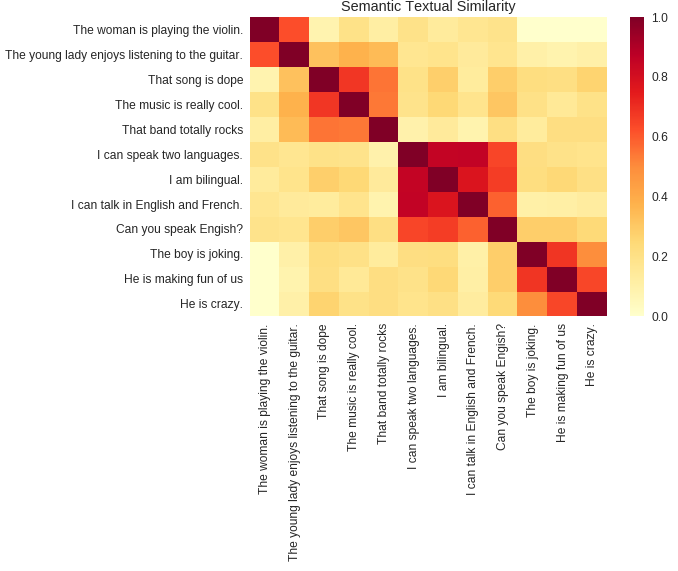
\includegraphics[width=0.8\textwidth]{sentence_similarity.png}
%        \caption{Using Google's universal sentence encoder, sentences are embedded and their similarity visualised. The colour of the field at (row, column) indicates the similarity between the sentence labels at (row, column). A darker colour indicates a stronger similarity.}
%        \label{fig:sentence similarity}
%    \end{figure}
%    Using \gls{utterance} embeddings, similar sentences can be clustered together, forming topics. A visual example showing sentence similarity is shown in Fig. \ref{fig:sentence similarity}.
%    Going through the transcript, once the cluster to which a sentence is assigned changes, a topic boundary is set. This theoretically allows for topic segmentation.
%
%    \subsubsection{Minimum Cut Graph Based \label{method: minimum cut}}
%
%        Firstly we evaluate the minimum cut based clustering method detailed in Sec. \ref{fig: graph seg} for conversations, in which all \glspl{utterance} above some threshold similarity are clustered. The key limitation within the context of conversation is that certain \glspl{utterance} appear within all topics. Consider the following sample of \glspl{utterance}:
%        \begin{table}[h]
%            \begin{tabular}{l|l}
%            $u_1$     & \textit{Rock music is the best!}                        \\
%            $u_2$     & \textit{Yeah man, rock is the best!}                    \\
%            \dots      &                                                         \\
%            $u_i$     & \textit{Lord of the Rings is the best movie ever made.} \\
%            $u_{i+1}$ & \textit{Yeah dude, Lord of the Rings really is the best.}              \\
%            \end{tabular}
%        \end{table}
%
%        Even though $u_1$ and $u_{i}$ correctly do not connect, $u_1$ connects to $u_2$, $u_{i}$ connects to $u_{i+1}$ and critically, $u_2$ connects to $u_{i+1}$. This last connection is made because the sentences are similar, in fact everything \textit{except for the topic} matches between these \glspl{utterance}. In conversation, sentences like $u_2$ and $u_{i+1}$ are abundant - leading to one giant connected component, which is a cluster that contains a large fraction of all nodes. We attempted to fine-tune the cutoff similarity, but either (almost) no sentences end up connected or all of them do.
%        From testing the method, we thus qualitatively identify two issues:
%        \begin{enumerate}
%            \item Sentences in conversation often carry little meaning, particularly those only acknowledge/agree with previous \glspl{utterance}. These acknowledgements act as bridges between clusters.
%            \item The minimum cut clustering method amplifies this because one \gls{utterance} acting as a bridge suffices to connect two clusters.
%        \end{enumerate}
%
%        The first issue is the key problem with using \gls{utterance} embeddings. While the minimum cut method is particularly vulnerable, other clustering methods also suffer from it.
%
%    \subsubsection{Other Clustering Methods}
%        Since the cutoff-based approach lead to issues, we try the following clustering methods in an attempt to minimize the vulnerability to falsely merged clusters:
%        \begin{itemize}
%            \item k-means clustering, in which the algorithm tries to separate samples in k groups of equal variance.
%            \item DBSCAN clustering, in which clusters are viewed as areas of high density separated by areas of low density.
%            \item Agglomerative clustering, in which a hierarchy of clusters is formed by assigning each \gls{utterance} its own cluster and then repeatedly merging the most similar clusters.
%        \end{itemize}
%        All three clustering methods were implemented using the python library scikit-learn\cite{scikit-learn}. These clustering methods qualitatively perform better than the minimum cut method, but each suffer from new issues. In k-means, imposing the number of topics $k$ is difficult as it varies heavily from conversation to conversation. In DBSCAN clustering, which requires neither a cutoff nor a number of topics, if data points are not inherently clustered (i.e. separated by areas of low density), the algorithm fails. This occured for a significant fraction of \glspl{utterance}. The most promising algorithm for clustering was the agglomerative clustering method, in which some topics could be clearly identified, but qualitative results were too poor to warrant further development and quantitative evaluation.
%
%    \subsubsection{Limitations}
%        No matter the clustering method, using sentence \glspl{embedding} is ineffective when analysing conversation topics. Some words in sentences don't contribute to the meaning act as unwanted bridges to other topics, but they can also \textit{dilute} the embedding. Consider the \glspl{utterance}
%
%
%        \begin{table}[h]
%            \begin{tabular}{l|l}
%            $u_1$     & \textit{Do you have any pets?}                    \\
%            $u_2$     & \textit{We had a light brown cat as a family pet when I was younger, but I don't now.}                        \\
%            \end{tabular}
%        \end{table}
%
%        Both \glspl{utterance} are about pets, but because the question and answer share almost no other words, and because the answer is very long, the sentences are deemed dissimilar by the \gls{model}. %TODO: actually get the sim value
%
%
%        % Put this as limitation in TopicRank
%        Another issue is that key-words are often not repeated but still understood as the topic. Consider the following \glspl{utterance}:
%
%        \begin{table}[h]
%            \begin{tabular}{l|l}
%            $u_1$     & \textit{Do you have any pets?}                    \\
%            $u_2$     & \textit{Yeah I've got a cat.}                        \\
%            \end{tabular}
%        \end{table}
%
%        The word ``pet" is not repeated  but from the context of the conversation it is clear that the topic is still ``pets".
%
%        The issue with the \gls{utterance} \gls{embedding} approach can be succinctly summarised as the following: \Glspl{Utterances} are more than just their topics. While the similarity of \glspl{utterances} is correlated with the similarity of the topics in which they lie, they are not equivalent. To make a more effective algorithm, the words representing topics must be first extracted.
%
%\subsection{Latent Dirichlet Allocation - BayesSeg \label{method: LDA}}
%    \begin{table}[]
%    \centering
%    \begin{tabular}{lllll}
%    \hline
%    \textbf{Topic 1}   & \textbf{Topic 2}    & \textbf{Topic 3}   & \textbf{Topic 4} & \textbf{Topic 5}  \\ \hline
%    technology   & models        & speakers     & wouldn't   & v\_a\_d     \\
%    u\_m\_t\_s   & reverberation & overlaps     & you'd      & worse       \\
%    routing      & voicing       & alignment    & agree      & t\_i-digits \\
%    transmission & multi-band    & region       & matter     & baseline    \\
%    i\_p         & targets       & breath       & depends    & I\_d\_a     \\
%    mobile       & phonemes      & laugh        & open       & percent     \\
%    packet       & effects       & native       & others     & italian     \\
%    university   & echo          & backchannels & feeling    & improvement \\
%    concerning   & combining     & laughing     & term       & adaptation  \\
%    networking   & insertions    & marks        & opposed    & latency     \\ \hline
%    \end{tabular}
%    \caption{Sample topics from recorded meeting dialogues, extracted by the modified \gls{lda} algorithm by Purver et al.\cite{purver2006unsupervised}. Words within topics are vaguely related, such as topic 1 concerning networking technology, or topic 3 about \glspl{da}. However, a lot of words don't fit well together and are unlikely to represent a topic.}
%    \label{table: modified lda topics}
%    \end{table}
%
%    One method of segmentation that attempts to extract topic-words is the modified \gls{lda} method \textit{BayesSeg} proposed by Eisenstein et al.\cite{eisenstein2008bayesian} (see Sec. \ref{ssec: topic segmentation}). We choose this method over the similar method presented by Purver et al.\cite{purver2006unsupervised}, because BayesSeg can be applied to individual documents, while the segmentation method by Purver et al. requires a whole corpus of documents. We only received access to the Spotify podcast corpus shortly before the date of submission of this thesis and so could not evaluate said method. However, from the examples shown in the original paper by Purver et al.\cite{purver2006unsupervised}, shown in Table \ref{table: modified lda topics}, we believe the algorithms suffer from similar limitations.
%
%    BayesSeg achieves the WindowDiff penalty score
%    \begin{equation}
%     w_d = 0.39 \pm 0.06
%    \end{equation}
%    when segmenting our annotated transcripts. The uncertainty is quite high because we had to annotate evaluation data manually, which is a time-consuming process and was thus limited to 4 transcripts. This is a significantly worse score than the value reported for the ICSI-MRDA corpus, $w_d = 0.312$\cite{eisenstein2008bayesian}.
%
%    While the results could agree due to the high uncertainty, we hypothesise the following reason for this reduction in performance instead: \gls{lda} assumes that every word is generated by sampling a topic, which is a distribution over words. Every word is assumed to be part of a topic. In more robust media, such as scientific papers or newspaper articles, this may be an appropriate approximation: if the aim is to convey information efficiently, most words will be related to the topic that is discussed. To an extent, the formal business meetings in the ICSI-MRDA corpus still fit this description. In more casual conversations, however, a lot of words are not related to the topic discussed: they act as statements of politeness, as acknowledgements, to fill breaks of awkward silence or to be entertaining\cite{searle1965speech}. This could be an explanation for the worse performance of BayesSeg in casual conversations, and could be further investigated in future work by evaluating performance on more and less formal conversations.
%
%      We identify two further key issues with \gls{lda}-based methods for casual conversation and use examples from the segmentation \gls{model} by Purver et al., shown in Table \ref{table: modified lda topics}, to support them:
%    \begin{enumerate}
%        \item The lack of correlations captured by \gls{lda} as well as its inability to \gls{model} temporal topic evolution means that unrelated topics can be falsely grouped together. For example ``university" does not fit in Topic 1, and ``Italy" does not fit in Topic 5.
%        \item The generative assumption that every word describes a topic leads to topics of words that do not have coherent semantic meaning and appear frequently, reducing the effectiveness of segmentation. An example is Topic 4.
%    \end{enumerate}
%
%
%    %TODO: lda cant do correlations, if two different topics appear together, it sticks them together (t2, t3, t5 (italian)).
%    %Also: forcing every word to belong to topic leads to misfits e.g. "combining" in 2, "concerning" in 1,
%
%\subsection{TopicRank \label{method: topic rank}}
%
%Utterance embedding based methods (Sec. \ref{method: utterance embedding clustering}) as well as \gls{lda}-based methods (Sec. \ref{method: LDA} are somewhat ineffective for the segmentation of conversation in part because they assume that every word in every \gls{utterance} contributes to the topic of the conversation, which is false.
%TopicRank\cite{bougouin-etal-2013-topicrank} (see Sec. \ref{ssec: keyphrase extraction}) offers a promising alternative approach: it first extracts \glspl{keyphrase} that are likely to represent topics and discards the rest.
%
%\subsubsection{Evaluation}
%We use TopicRank on our hand-annotated transcripts and compare its selected topic-phrases against human-annotated topic-phrases. If a topic-phrase extracted by TopicRank, $t_{\text{TR}}$ has a similarity greater than

\section[Clustering]{Utterance Embedding Clustering \label{method: utterance embedding clustering}}
    \begin{figure}[t]
        \centering
        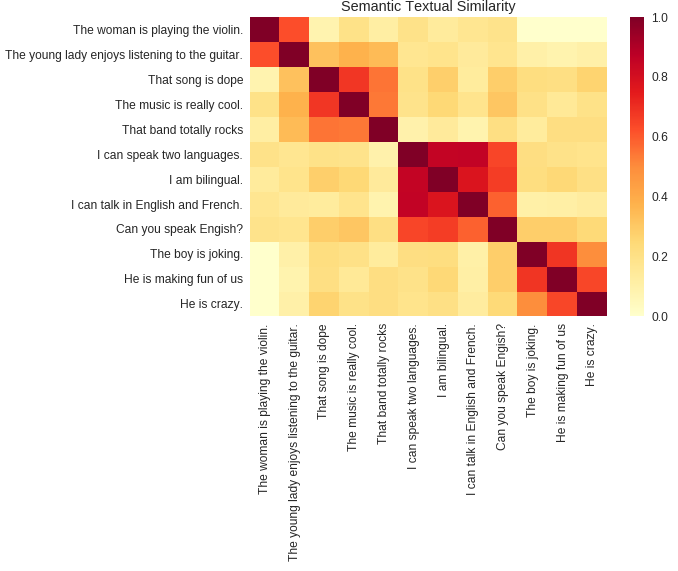
\includegraphics[width=0.8\textwidth]{sentence_similarity.png}
        \caption{Using Google's universal sentence encoder, sentences are embedded and their similarity visualised. The colour of the field at (row, column) indicates the similarity between the sentence labels at (row, column). A darker colour indicates a stronger similarity.}
        \label{fig:sentence similarity}
    \end{figure}
    As a first topic segmentation approach, we follow the graph-based technique introduced by Malioutov et al.\cite{malioutov2006minimum} (see Sec. \ref{ssec: topic segmentation}). Using \gls{utterance} \glspl{embedding} to cluster semantically similar sentences, forming topics. Going through the transcript, once the cluster to which a sentence is assigned changes, a topic boundary is set. This theoretically allows for topic segmentation. A visual example showing clusters of similar sentences is shown in Fig. \ref{fig:sentence similarity}.

    \subsection{Minimum Cut Graph Based \label{method: minimum cut}}

        Firstly we evaluate the minimum cut based clustering method detailed in Sec. \ref{fig: graph seg} for conversations, in which all \glspl{utterance} above some threshold similarity are clustered.
        
        Unfortunately, this approach does not work well: The key limitation within the context of conversation is that certain \glspl{utterance} appear within all topics. Consider the following sample of \glspl{utterance}:
        \begin{table}[h]
            \begin{tabular}{l|l}
            $u_1$     & \textit{Rock music is the best!}                        \\
            $u_2$     & \textit{Yeah man, rock is the best!}                    \\
            \dots      &                                                         \\
            $u_i$     & \textit{Lord of the Rings is the best movie ever made.} \\
            $u_{i+1}$ & \textit{Yeah dude, Lord of the Rings really is the best.}              \\
            \end{tabular}
        \end{table}

        \Glspl{utterance} $u_1$ and $u_2$ connect, $u_{i}$ connects to $u_{i+1}$ and even though $u_1$ and $u_{i}$ correctly do not connect, $u_2$ mistakenly connects to $u_{i+1}$. \color{red} \textbf{TODO: get values}. \color{black} This last connection is made because the sentences are similar, in fact everything \textit{except for the topic} matches between these \glspl{utterance}. In conversation, sentences like $u_2$ and $u_{i+1}$ are abundant --- leading to one giant connected component (a cluster that contains a large fraction of all nodes). We attempted to fine-tune the cutoff similarity, but either (almost) no sentences end up connected or all of them do.


    \subsection{Other Clustering Methods}
        Since the cutoff-based approach lead to issues, we try the following clustering methods in an attempt to minimise the vulnerability to falsely merged clusters:
        \begin{itemize}
            \item k-means clustering, in which the algorithm tries to separate samples in k groups of equal variance.
            \item DBSCAN clustering, in which clusters are viewed as areas of high density separated by areas of low density.
            \item Agglomerative clustering, in which a hierarchy of clusters is formed by assigning each \gls{utterance} its own cluster and then repeatedly merging the most similar clusters.
        \end{itemize}
        All three clustering methods were implemented using the python library scikit-learn\cite{scikit-learn}. While some clustering methods (especially agglomerative clustering) qualitatively perform better than the minimum cut method, none work well enough to warrant time-consuming quantitative evaluation.

        %These clustering methods qualitatively perform better than the minimum cut method, but each suffer from new issues. In k-means, imposing the number of topics $k$ is difficult as it varies heavily from conversation to conversation. In DBSCAN clustering, which requires neither a cutoff nor a number of topics, if data points are not inherently clustered (i.e. separated by areas of low density), the algorithm fails. This occured for a significant fraction of \glspl{utterance}. The most promising algorithm for clustering was the agglomerative clustering method, in which some topics could be clearly identified, but qualitative results were still too poor to warrant further development and quantitative evaluation.

    \subsection{Limitations}
        No matter the clustering method, using sentence \glspl{embedding} is ineffective when analysing conversation topics. \Glspl{utterance} in casual conversations are more than just their topics, many words dilute the semantics of an \gls{utterance} to such an extent that it becomes
        \begin{enumerate}
            \item indistinguishable from other \glspl{utterance} talking about different topics
            \item too dissimilar to other \glspl{utterance} talking about the same topic
        \end{enumerate}
        making it a poor method for topic segmentation.


        %A lot of words Some words in sentences don't contribute to the meaning act as unwanted bridges to other topics, but they can also \textit{dilute} the embedding. Consider the \glspl{utterance}


        %\begin{table}[h]
        %    \begin{tabular}{l|l}
        %    $u_1$     & \textit{Do you have any pets?}                    \\
        %    $u_2$     & \textit{Yeah, well, we had a light brown cat when I was younger, but I don't now.}                        \\
        %    \end{tabular}
        %\end{table}

        %Both \glspl{utterance} are about pets, but because the question and answer share almost no other words, and because the answer is very long, the sentences are deemed dissimilar by the model. %TODO: actually get the sim value



        %The issue with the \gls{utterance} \gls{embedding} approach can be succinctly summarised as the following: \Glspl{utterance} are more than just their topics. While the similarity of \glspl{utterance} is correlated with the similarity of the topics in which they lie, they are not equivalent. To make a more effective algorithm, the words representing topics must be first extracted.

\section[LDA BayesSeg]{Latent Dirichlet Allocation - BayesSeg \label{method: LDA}} 
    \begin{table}[]
    \centering
    \begin{tabular}{lllll}
    \hline
    \textbf{Topic 1}   & \textbf{Topic 2}    & \textbf{Topic 3}   & \textbf{Topic 4} & \textbf{Topic 5}  \\ \hline
    technology   & models        & speakers     & wouldn't   & v\_a\_d     \\
    u\_m\_t\_s   & reverberation & overlaps     & you'd      & worse       \\
    routing      & voicing       & alignment    & agree      & t\_i-digits \\
    transmission & multi-band    & region       & matter     & baseline    \\
    i\_p         & targets       & breath       & depends    & I\_d\_a     \\
    mobile       & phonemes      & laugh        & open       & percent     \\
    packet       & effects       & native       & others     & italian     \\
    university   & echo          & backchannels & feeling    & improvement \\
    concerning   & combining     & laughing     & term       & adaptation  \\
    networking   & insertions    & marks        & opposed    & latency     \\ \hline
    \end{tabular}
    \caption{Sample topics from recorded meeting dialogues, extracted by the modified LDA algorithm by Purver et al.\cite{purver2006unsupervised}. Words within topics are vaguely related, such as topic 1 concerning networking technology, or topic 3 about conversations. However, a lot of words don't fit well together and are unlikely to represent a topic.}
    \label{table: modified lda topics}
    \end{table}
    
    One method of segmentation that attempts to extract topic-words is the modified LDA method \textit{BayesSeg} proposed by Eisenstein et al.\cite{eisenstein2008bayesian} (see Sec. \ref{ssec: topic segmentation}). We choose this method over the similar method presented by Purver et al.\cite{purver2006unsupervised}, because BayesSeg can be applied to individual documents, while the segmentation method by Purver et al. requires a whole corpus of documents. We only received access to the Spotify podcast corpus shortly before the date of submission of this thesis and so could not evaluate said method. However, from the examples shown in the original paper by Purver et al.\cite{purver2006unsupervised}, shown in Table \ref{table: modified lda topics}, we believe the algorithms suffer from similar limitations.
    
    BayesSeg achieves the WindowDiff penalty score
    \begin{equation}
     w_d = 0.39 \pm 0.06
    \end{equation} 
    when segmenting our annotated transcripts. The uncertainty is quite high because we had to annotate evaluation data manually, which is a time-consuming process and was thus limited to 4 transcripts. This is a significantly worse score than the value reported for the ICSI-MRDA corpus, $w_d = 0.312$\cite{eisenstein2008bayesian}.
    
    We hypothesis that the reduction in performance comes from the change in media: we believe podcast conversations to be more casual, less topic-oriented (less expert knowledge) and less structured than dialogue in meetings, leading to a more difficult segmentation.
    
    %While the results could agree due to the high uncertainty, we hypothesise the following reason for this reduction in performance instead: LDA assumes that every word is generated by sampling a topic, which is a distribution over words. Every word is assumed to be part of a topic.
    %In more robust media, such as scientific papers or newspaper articles, this may be an appropriate approximation: if the aim is to convey information efficiently, most words will be related to the topic that is discussed.
    %To an extent, the formal business meetings in the ICSI-MRDA corpus still fit this description, sentences in meetings are trying to convey information efficiently, they largely relate to the topic at hand. In more casual conversations, however, a lot of words are not related to the topic discussed: they act as statements of politeness, as acknowledgements, to fill breaks of awkward silence or to be entertaining\cite{searle1965speech}.
    %This could be an explanation for the worse performance of BayesSeg in casual conversations, and could be further investigated in future work by evaluating performance on more and less formal conversations.
    
      We identify two further key issues with LDA-based methods for casual conversation and use examples from the segmentation model by Purver et al., shown in Table \ref{table: modified lda topics}, to support them:
    \begin{enumerate}
        \item The lack of correlations captured by LDA as well as its inability to model temporal topic evolution means that unrelated topics can be falsely grouped together. For example ``university" does not fit in Topic 1, and ``Italy" does not fit in Topic 5.
        \item The generative assumption that every word describes a topic leads to topics of words that do not have coherent semantic meaning and appear frequently, reducing the effectiveness of segmentation. An example is Topic 4.
    \end{enumerate}
    
    
    %TODO: lda cant do correlations, if two different topics appear together, it sticks them together (t2, t3, t5 (italian)). 
    %Also: forcing every word to belong to topic leads to misfits e.g. "combining" in 2, "concerning" in 1, 
\section{TopicRank \label{method: topic rank}}

Utterance \gls{embedding} based methods (Sec. \ref{method: utterance embedding clustering}) as well as \gls{lda}-based methods (Sec. \ref{method: LDA} are somewhat ineffective for the segmentation of conversation in part because they assume that every word in every \gls{utterance} contributes to the topic of the conversation, which is false.
TopicRank\cite{bougouin-etal-2013-topicrank} (see Sec. \ref{ssec: keyphrase extraction}) offers a promising alternative approach: it first extracts \glspl{keyphrase} that are likely to represent topics and discards the rest.

\subsection{Evaluation}
\begin{figure}
    \centering
    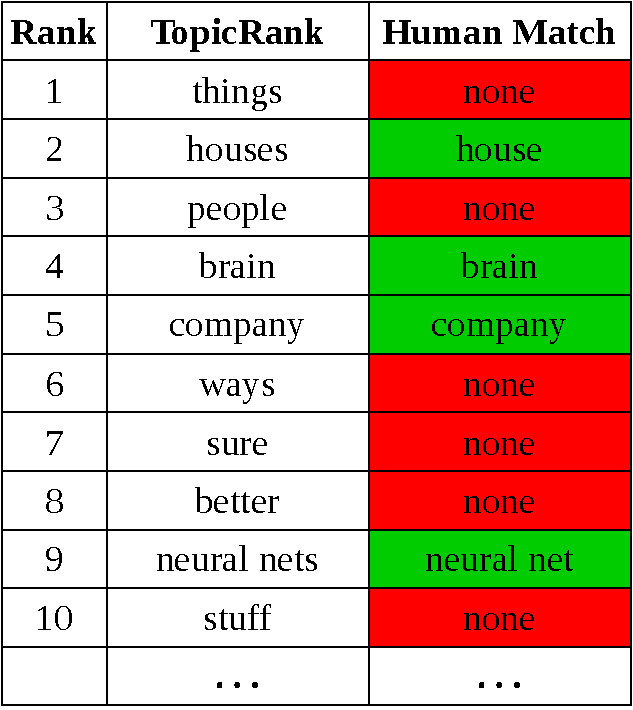
\includegraphics[width=0.5\textwidth]{topicRankEval.pdf}
    \caption{Top 10 \glspl{keyphrase} as determined by TopicRank and human matches where appropriate.}
    \label{fig: topicrank eval}
\end{figure}
We use TopicRank on our hand-annotated transcripts and compare its selected topic-phrases against human-annotated topic-phrases. If a given transcript has $N_{h}$ human annotated \glspl{keyphrase}, the top $N_{h}$ \glspl{keyphrase} as determined by the TopicRank algorithm are extracted. If a \gls{keyphrase} extracted by TopicRank or its plural/singular version is also found to be a \gls{keyphrase} by the human annotator, it is a match. On the 4 annotated transcripts, TopicRank achieves an accuracy (i.e. overlap with human \glspl{keyphrase})
\begin{equation}
    \text{accuracy} = 0.45 \pm 0.20.
    \label{eq: topic rank accuracy}
\end{equation}

\subsection{Limitations}
Fig. \ref{fig: topicrank eval} shows the top 10 highest ranked \glspl{keyphrase} and its human annotated counterpart if it exists. This illustrates two limitations of TopicRank:
\begin{enumerate}
    \item Abstract nouns such as ``things", ``people" or ``ways" are identified as topics even though they do not indicate a topic.
    \item Adjectives that are included as \gls{keyphrase} candidates, such as ``better" most often do not indicate a topic.
\end{enumerate}

% Put this as limitation in TopicRank
Another issue is that key-words are often not repeated but still understood as the topic. Consider the following \glspl{utterance}:

\begin{table}[h]
    \begin{tabular}{l|l}
    $u_1$     & \textit{Do you have any pets?}                    \\
    $u_2$     & \textit{Yeah I've got a cat.}                        \\
    \end{tabular}
\end{table}

The word ``pet" is not repeated  but from the context of the conversation it is clear that the topic is still ``pets". To improve the topic matching, we thus need to match semantically \textbf{similar} words instead of just matching equal words.

\section{GEEK Algorithm}

    \begin{figure}
        \centering
        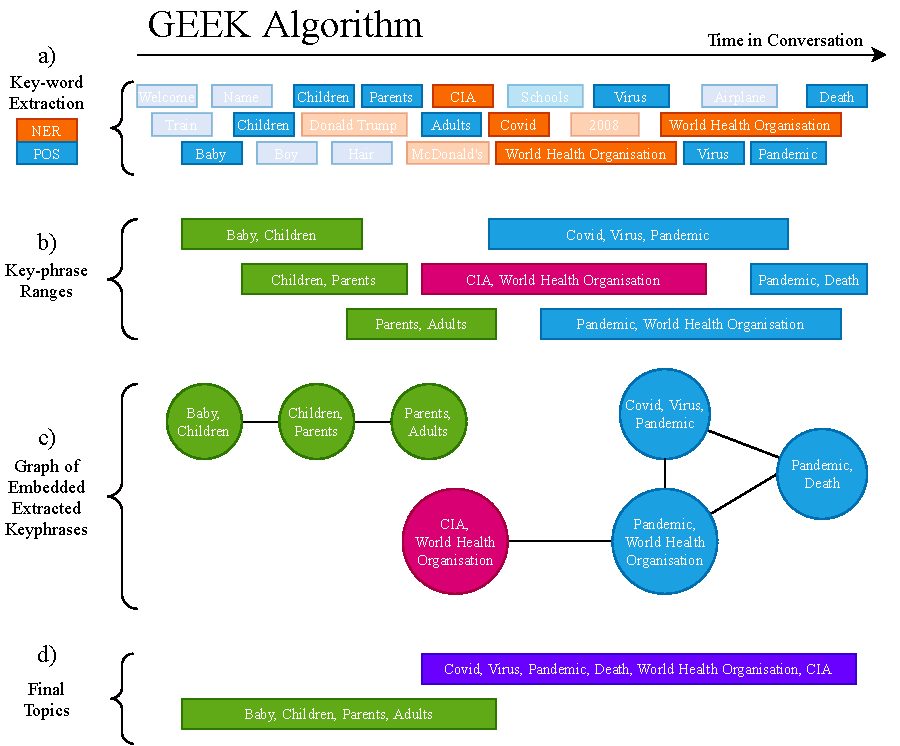
\includegraphics[width=\textwidth]{geek.pdf}
        \caption{A toy example showing how GEEK works.\newline a) \Glspl{keyphrase} are extracted as nouns and proper nouns using \gls{pos} tagging (blue) and as named entities using \gls{ner} (orange). The words on a transparent background are discarded because they are not similar to other nearby \glspl{keyphrase}.\newline b) The \glspl{keyphrase} are matched with similar nearby \glspl{keyphrase} and the range of their effect is determined. \newline c) A graph of \glspl{keyphrase} is created based on \gls{keyphrase}-range overlap and similarity. The colour is meant to serve as a visualisation of embeddings (similar colour $\rightarrow$ similar embedding).\newline
        d) The topics are the \glspl{keyphrase} in connected components in the graph. They range from the earliest \gls{keyphrase} occurence to the latest. The meaning of the final topic is influenced by all connected \glspl{keyphrase} (shown here as colour mixing).
        }
        \label{fig:geek architecture}
    \end{figure}

We use the TopicRank approach and build upon it to develop an algorithm that both segments and labels topics. We call this improved algorithm the \gls{geek} algorithm. \gls{geek} extracts \glspl{keyphrase}, but uses different criteria to make a different selection than TopicRank.
It then uses \gls{embedding}-based similarity to determine cohesive sections of the transcript. An example of how \gls{geek} works is shown in Fig. \ref{fig:geek architecture}.

\gls{geek} is based on the following assumptions:

\begin{enumerate}
    \item Topics are described by a small number of \glspl{keyphrase}. We assume \glspl{keyphrase} to exclusively be nouns, proper nouns and named entities, such as \textit{family}, \textit{music}, \textit{Donald Trump, the CIA} or \textit{Tesla}.
    \item Topics are sections within the text that feature similar \glspl{keyphrase}. \glspl{keyphrase} that are only mentioned once can not represent a topic.
    \item There can be more than one active topic: topics can overlap and smaller sub-topics can be discussed within larger topics.
    \item If the gap between related \glspl{keyphrase} is too large, they do not belong to the same segment.
\end{enumerate}
    
    \vbox{ %don't pagebreak this.
        \subsection{Hyperparameters}
        The hyperparameters that the user needs to set to use \gls{geek} are as follows:
        
        \newcolumntype{t}{>{\hsize=.15\hsize}X}
        \newcolumntype{L}{>{\hsize=.7\hsize}X}
        \begin{table}[H]
            \centering
            \begin{tabularx}{0.9\textwidth}{| t | L | t |}
            \hline
            \textbf{Symbol} & \textbf{Description} & \textbf{Chosen Value} \\ \hline
            $\Delta_{\text{max}}$     & The maximum gap between matching \glspl{keyphrase} for them to be considered in the same segment & 11                    \\ \hline
            $\eta_{\text{min}}$     & The minimum cosine similarity of two word \glspl{embedding} for their words to be considered similar. & 0.55                        \\ \hline
            $T_{\text{min}}$ & Minimum number of \glspl{utterance} a topic must span. & 3 \\ \hline
    
            \end{tabularx}
        \end{table}
    }
    

    \subsection{Keyword Extraction}
        TopicRank extracts noun phrases such as
        \begin{equation*}
            ``\textbf{The spotted puppy}\text{ is up for adoption.}",
        \end{equation*}
        as \glspl{keyphrase}. We instead only extract the nouns, proper nouns and named entities themselves (and no surrounding adjectives/articles). We do this because most multi-word noun phrases do not have pre-trained \glspl{embedding}. However, if a two-word phrase ends in a noun and is a part of the \glspl{embedding} it is also added as a \gls{keyphrase} to include phrases such as ``neural net" and ``absolute zero". The \glspl{embedding} used here are the \textit{\gls{numberbatch} mini} \gls{embedding} (which sacrifice a little bit of accuracy for much smaller filesizes). The \gls{keyphrase} extraction process is shown in Fig. \ref{fig:geek architecture} a).

        \subsubsection{POS Tagging}
            We extract \gls{pos} tags using the pre-trained state of the art \gls{pos} tagger by the python library Flair\cite{flairNLP}. It tags every word with its grammatical function and allows us to extract nouns and proper nouns (see Sec. \ref{sssec: POS tagging}).

        \subsubsection{Named Entity Recognition}
            We also use the pre-trained state of the art \gls{ner} tagger from the python library Flair\cite{flairNLP}.
            \Gls{ner} taggers can be written as \glspl{model}:
            \begin{equation}
              \hat{f}_{\text{ner}}: S \rightarrow W_{\text{ne}},
            \end{equation}
            that extract a set of words $W_{\text{ne}}$ from sequences of words $S$ that describe a named entity such as a person, company or date and label them accordingly. For example:
        \begin{align*}
        \text{[Bill Gates, founded, Microsoft, in, 1975]} \rightarrow [& (\text{Bill Gates, person}), \\
                                                                       & (\text{Microsoft, company}), \\
                                                                       & (\text{1975, year})].
        \end{align*}
        This tagging problem is approached almost exactly like the \gls{da} tagging from Sec. \ref{ssec: da classification}, and allows us to extract named entities as \glspl{keyphrase}\cite{flairNLP}.

        \subsubsection{Post Processing}
            Some words are technically nouns but are unwanted as \glspl{keyphrase}. They include words such as ``dude", ``everything" or ``dope". We manually exclude 89 such words $\mathcal{W}_{man}$ from the \glspl{keyphrase} and also exclude any words that are similar enough to any $w_{man} \in \mathcal{W}_{man}$, where similarity is defined as usual as the cosine similarity of two word \glspl{embedding} and $0.9$ is the minimum cosine similarity for exclusion.

    \subsection{Determining Keyword Ranges}
        After we extract \glspl{keyphrase}, we determine the range of \glspl{utterance} over which it is ``active" (see Fig. \ref{fig:geek architecture} b)). We do this by starting at the \gls{utterance} containing a \gls{keyphrase} $u_i$ and searching the next $\Delta_{\text{max}}$ \glspl{utterance} for matches, where matches are defined as \glspl{keyphrase} whose \glspl{embedding} $\mathbf{w_i}, \mathbf{w_j}$ have a similarity
        \begin{equation}
            \text{cosine}(\mathbf{w_i}, \mathbf{w_j}) \geq \eta_{\text{min}}.
        \end{equation}
        If a match is found at \gls{utterance} $u_j$, the search is repeated with the \textbf{same \gls{keyphrase}}, this time starting from $u_j$. This is repeated until no match is found. Then the end of the range is defined to be the last occurrence of a match. If the range is smaller than $T_{\text{min}}$, the range is discarded.

    \subsection{Joining Topic Ranges}
        Now the \gls{keyphrase} ranges are joined so that similar overlapping \glspl{keyphrase} are joined. To do this, all \gls{keyphrase} ranges $k_i$ are represented as nodes in a Graph. Two nodes $k_i$ and $k_j$ are connected if $k_i$ and $k_j$ match and if the ranges of $k_i$ and $k_j$ overlap. We essentially follow the minimum cut procedure discussed in Sec. \ref{method: utterance embedding clustering}, but instead of sentences, we cluster overlapping \glspl{keyphrase}. The clustered $k_i$ represent the final topic labels, their ranges determine the final segmentation. This process is illustrated in Fig. \ref{fig:geek architecture} c) and d). An example of the final outcome (applied to a real conversation transcript) that shows many of \gls{geek}'s features is visualised in Fig. \ref{fig:GEEK final result}.

        \begin{figure}
            \centering
            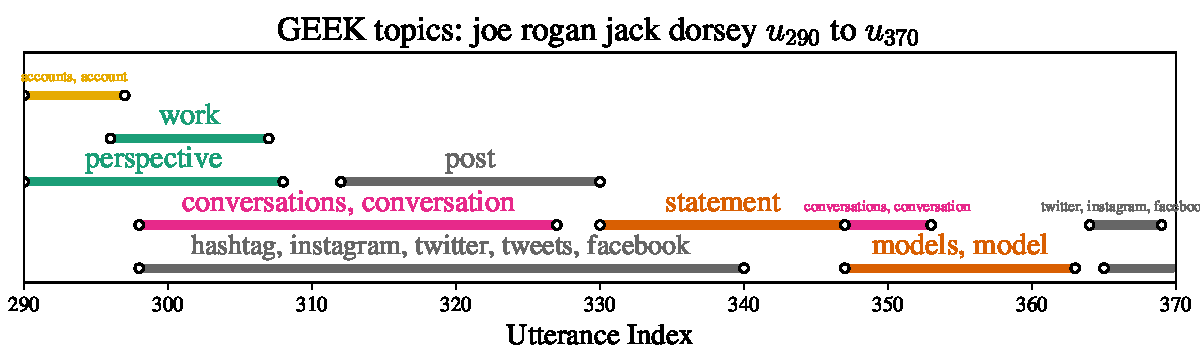
\includegraphics[width=\textwidth]{joe_rogan_jack_dorsey290_370_topics.pdf}
            \caption{The extracted topics within an excerpt of a conversation between podcast host Joe Rogan and twitter CEO Jack Dorsey. The y-axis is used to display simultaneous topics. Similar \glspl{keyphrase} are grouped together into topics. Topics are colour-coded by mapping \glspl{embedding} to a colour.}
            \label{fig:GEEK final result}
        \end{figure}

    \subsection{Evaluation}

    \subsubsection{Segmentation}
        Even though segmentation is not exactly possible as there are multiple topics that may overlap, by simply placing a topic boundary at the start of the largest topic out of a group of overlapping topics, we can achieve a reasonable approximation. This is visualised in Fig. \ref{fig:GEEK segment}.
        \begin{figure}
             \centering
             \begin{subfigure}[b]{\textwidth}
                 \centering
                 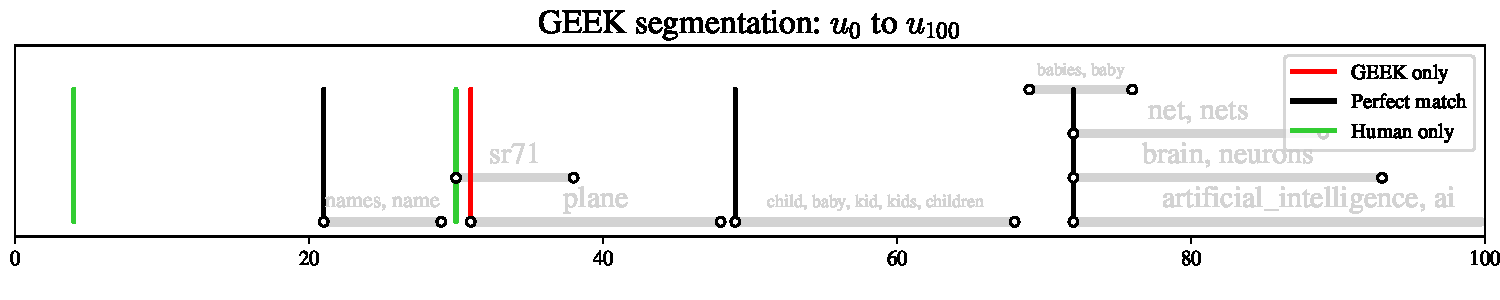
\includegraphics[width=1\textwidth]{figures/0to100segment_topics.pdf}
                 \caption{$u_0$ to $u_{100}$}
             \end{subfigure}
             \hfill
             \begin{subfigure}[b]{\textwidth}
                 \centering
                 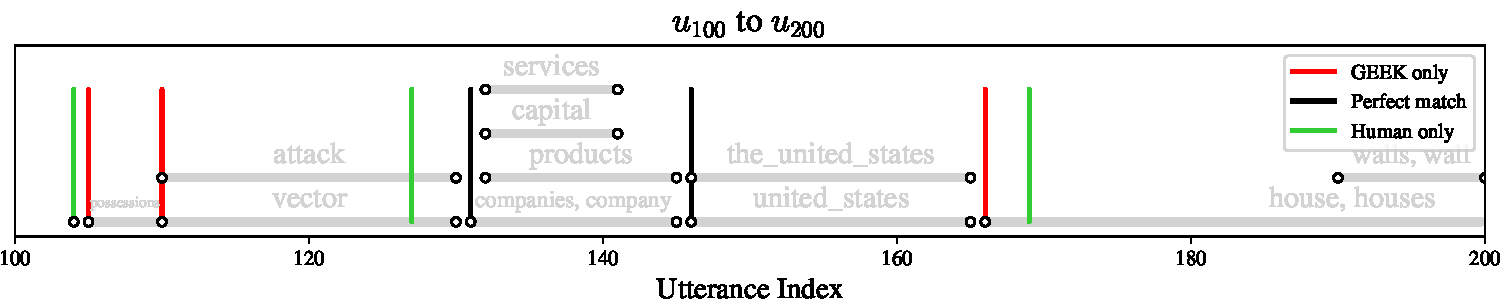
\includegraphics[width=1\textwidth]{figures/100to200segment_topics.pdf}
             \end{subfigure}
                \caption{200 \glspl{utterance} out of the evaluation transcript of a conversation between host Joe Rogan and guest Elon Musk. Vertical lines indicate boundaries: Green lines indicate human boundaries, red lines indicate boundaries placed by \gls{geek} and black lines are boundaries where the two agree exactly. Most boundaries are exactly or approximately detected by \gls{geek}. Failures include $u_4$ (missed topic change) or $u_{110}$ (false boundary).}
                \label{fig:GEEK segment}
        \end{figure}

        Using this approximation, \gls{geek} achieves a state of the art windowDiff score of
        \begin{equation}
            w_d = 0.22 \pm 0.04.
        \end{equation}


    \subsubsection{Labelling}
        We evaluate extracted topic labels in the same way we evaluated TopicRank \glspl{keyphrase} (Sec. \ref{method: topic rank}), with the small modification that multi-word topics match if any constituent words match the human annotation. This modification is small because multi-word topics already contain very similar words. \gls{geek} achieves an accuracy of
        \begin{equation}
            0.72 \pm 0.12,
        \end{equation}
        which is a significant improvement over TopicRank (see Eq. \ref{eq: topic rank accuracy}). It should be noted that only one author annotated selected \glspl{keyphrase}, which is a subjective task. It is expected that \gls{geek}'s accuracy is thus somewhat biased as its assumptions align more with the author's assumptions than TopicRanks's do. In future work it would be preferable to have multiple human annotators which provides an insight into labelling uncertainty and provides a more objective evaluation.

    \subsection{Limitations}
    \gls{geek} still suffers from some limitations, that we briefly outline here.

    \subsubsection{False Keywords}
        Some words are nouns and are used in conversation but do not describe topics. While \gls{geek} is somewhat robust against this, by requiring \glspl{keyphrase} to appear at least twice at least $T_{\text{min}}$ \glspl{utterance} apart, sometimes it fails. An example is the phrase ``attack vector" that Elon Musk uses in the conversation shown in Fig. \ref{fig:GEEK segment}. This phrase is a non-standard way of saying ``point of weakness", but because Elon Musk, and eventually the host Joe Rogan, keep using it, it is detected by \gls{geek} as two \glspl{keyphrase} ``attack" and ``vector". This leads to a wrong segmentation (the red vertical line at $u_{110})$.

    \subsubsection{Missed Topics}
        In some cases \gls{geek} also suffers from the opposite issue: minimum topic length may discard some actual topics that happen to be over quickly. An example for that is a missed boundary at $u_4$ in Fig. \ref{fig:GEEK segment}.

    \subsubsection{Ambiguous Embeddings}
        Certain matches are not detected because words can not be disambiguated (see Sec. \ref{fig:ambiguous_embedding}). For example, in Fig. \ref{fig:GEEK final result}, the \gls{keyphrase} ``post" should be included in the topic ``hasthag, instagram twitter, tweets, facebook", because ``post" and ``tweets" should be considered similar. Unfortunately, the word ``post" has ambiguous meanings, which leads to a poor embedding. To fix this, newer transformer \glspl{embedding} such as ElMo\cite{peters2018elmo} or BERT\cite{devlin2018bert}, that make \glspl{embedding} context-dependent and thus disambiguated could be evaluated in future work. \newline

\glsresetall